\chapter{Experimental Setup}
\label{chap:methodology}
This chapter introduces the experimental setup for the works. 
First a description of the three HPC clusters and their characteristics 
on which we run our experiments is given.
Then the chapter provides information regarding the task-based parallel 
programming model and the two deep learning frameworks used in the work.
Finally we give a description of the datasets used.

\section{Hardware Platforms} 
Our experiments are run on four HPC clusters with distinct characteristics.  
They are the MareNostrum III and its upgrade MareNostrum IV supercomputer, 
MinoTauro supercomputer and CTE-POWER supercomputer at Barcelona Supercomputing 
Center (BSC). The results from the Iteration-Fusing Conjugate Gradient algorithm 
is evaluated on the MareNostrum III supercomputer. The evaluations of the deep 
neural networks are from the MinoTauro and CTE-POWER supercomputers. Their 
configurations are as follows:
\begin{itemize}
    \item \textit{MareNostrum III}: It consists of 3,065 compute nodes in total.  
        Each node is IBM System X server iDataPlex dx360 M4, composed of two 
        8-core Intel Sandy Bridge processors E5 - 2.60Hz, 20 MB of shared 
        last-level cache. There are eight 4GB DDR3 DIMM's running at 1.6 GHz (a 
        total of 32GB per node and 2BG per core).
    \item \textit{MareNostrum IV}: An upgrade to the \textit{MareNostrum III} 
        supercomputer. It consists of 3,456 compute nodes with a grand total of 
        165,888
        processor cores and 390 TB of main memory. Each node is Lenovo system 
        composed of SD530 Compute Racks, 2 sockets Intel Xeon Platinum 8160 CPU 
        with 24 cores each @ 2.10GHz for a total of 48 cores, 33 MB of shared 
        last-level cache, 96 GB of main memory 1.880 GB/core, 12x 8GB 2667Mhz 
        DIMM, 100 Gbit/s Intel Omni-Path HFI Silicon 100 Series PCI-E adapter.
    \item \textit{MinoTauro}: It is a heterogeneous cluster with 38 bullx 
        R421-E4 servers. Each server with 2 Intel Xeon E5 U2630 v3 (Haswell) 
        8-core processors, (each core at 2.4 GHz,and with 20 MB L3 cache), 2 K80 
        NVIDIA GPU Cards
        128 GB of Main memory, distributed in 8 DIMMs of 16 GB DDR4 @ 2133 MHz - 
        ECC SDRAM
        1 PCIe 3.0 x8 8GT/s, Mellanox ConnectX~\textregistered 3FDR 56 Gbit.
    \item \textit{CTE-POWER}: Another heterogeneous cluster with 52 compute 
        nodes. Each of which is equipped with 2 x IBM Power9 8335-GTH @ 2.4GHz 
        (3.0GHz on turbo, 20 cores and 4 threads/core, total 160 threads per 
        node).
        512 GB of main memory distributed in 16 dimms x 32 GB @ 2666MHz.  4 
        NVIDIA V100 (Volta) GPUs with 16 GB HBM2. Single Port Mellanox EDR.
\end{itemize}

\section{OmpSs Programming Model}
OmpSs is a programming model composed of a set of directives and library routines 
that can be used in conjunction with a high level programming language in order to 
develop concurrent applications. This programming model is an effort to integrate 
features from the StarSs programming model family, developed by the Programming 
Models group of the Computer Sciences department at Barcelona Supercomputing 
Center (BSC), into a single programming model.

OmpSs is based on tasks and dependences. Tasks are the elementary unit of work 
which represents a specific instance of an executable code. Dependences let the 
user annotate the data flow of the program, this way at runtime this information 
can be used to determine if the parallel execution of two tasks may cause data races.
In OmpSs the task construct also allows the annotation of function declarations or 
definitions in addition to structured-blocks. When a function is annotated with the 
task construct each invocation of that function becomes a task creation point.

The task construct allows expressing data-dependences among tasks using the 
\textit{in}, \textit{out} and \textit{inout} clauses (standing for input, output 
and input/Output respectively). They allow to specify for each task in the program 
what data a task is waiting for and signaling is readiness.

Each time a new task is created, its \textit{in} and \textit{out} dependences are 
matched against those of existing tasks. If a dependency, either RaW, WaW or WaR, 
is found the task becomes a successor of the corresponding tasks. This process 
creates a task dependency graph at runtime. Tasks are scheduled for execution as 
soon as all their predecessor in the graph have finished (which does not mean they 
are executed immediately) or at creation if they have no predecessors.

\section{Deep Learning Frameworks}
From a functionality-wise perspective, to construct a neural network boils down 
to stringing together a sequence of simple arithmetic functions. The derivatives
of such functions have to be computed when applying the backpropagation process.
Since the surge of deep learning, neural networks are getting deeper which means 
stacking up more layers. Each layer would have basically the same set of 
arithmetic functions. It soon becomes a redundant and error-prone procedure for 
a programmer to build a neural network from ground up every time. 

Software libraries that implement common arithmetic functions, perform auto-differentiation 
set off to alleviate the hassle. Such libraries are called deep learning frameworks 
and has become a common practice to build neural networks. Common frameworks are 
Keras, Theano, TensorFlow, PyTorch etc. These frameworks are usually build 
neural networks by constructing a computational graph that defines the type and 
sequence of operations prior to the actual computation.
In order to facilitate the development and debugging of building neural networks,
modern deep learning frameworks also encapsulate and expose APIs of the entire 
neural networks etc.

\subsection{Tensorflow}
TensorFlow is an open source software library for numerical computation using data 
flow graphs. The graph nodes represent mathematical operations, while the graph 
edges represent the multidimensional data arrays (tensors) that flow between them. 
This flexible architecture enables you to deploy computation to one or more CPUs or 
GPUs in a desktop, server, or mobile device without rewriting code. TensorFlow 
also includes TensorBoard, a data visualization toolkit. 

TensorFlow also takes a graph-based approach to construct neural networks in which 
each node in the graph represents an op. An op is a function that runs on the 
desired devices. Its functionality can thus be extended by adding customized ops 
using its C++ interface and API.

\subsection{KANN}
KANN is a standalone and lightweight library in C for constructing and training 
small to medium artificial neural networks such as multi-layer perceptrons, 
convolutional neural networks and recurrent neural networks (including LSTM and GRU). 
It implements graph-based reverse-mode automatic differentiation and allows to build 
topologically complex neural networks with recurrence, shared weights and multiple 
inputs/outputs/costs. In comparison to mainstream deep learning frameworks such as 
TensorFlow, KANN is not as scalable, but it is close in flexibility, has a much smaller 
code base and only depends on the standard C library. In comparison to other 
lightweight frameworks such as tiny-dnn, KANN is still smaller, times faster and 
much more versatile, supporting RNN, VAE and non-standard neural networks that 
may fail these lightweight frameworks.

\section{Datasets}
\subsection{SuiteSparse Matrix Collection}
The SuiteSparse Matrix Collection (formerly known as the University of Florida 
Sparse Matrix Collection), is a large and actively growing set of sparse 
matrices that arise in real applications. The Collection is widely used by the 
numerical linear algebra community for the development and performance 
evaluation of sparse matrix algorithms. It allows for robust and repeatable 
experiments: robust because performance results with artificially-generated 
matrices can be misleading, and repeatable because matrices are curated and made 
publicly available in many formats. Its matrices cover a wide spectrum of 
domains, include those arising from problems with underlying 2D or 3D geometry 
(as structural engineering, computational fluid dynamics, model reduction, 
electromagnetics, semiconductor devices, thermodynamics, materials, acoustics, 
computer graphics/vision, robotics/kinematics, and other discretizations) and 
those that typically do not have such geometry (optimization, circuit 
simulation, economic and financial modeling, theoretical and quantum chemistry, 
chemical process simulation, mathematics and statistics, power networks, and 
other networks and graphs). 

\subsection{CIFAR-10 dataset}
The CIFAR-10 dataset consists of 60000 32x32 color images in 10 classes, with 
6,000 images per class. There are 50,000 training images and 10,000 test images.
The dataset is divided into five training batches and one test batch, each with 
10000 images. The test batch contains exactly 1000 randomly-selected images from 
each class. The training batches contain the remaining images in random order, 
but some training batches may contain more images from one class than another. 
Between them, the training batches contain exactly 5000 images from each class.
Figure~\ref{fig:cifar10} illustrates the classes in the dataset, as well as 10 
random images from each.
\begin{figure}[H]
    \centerline{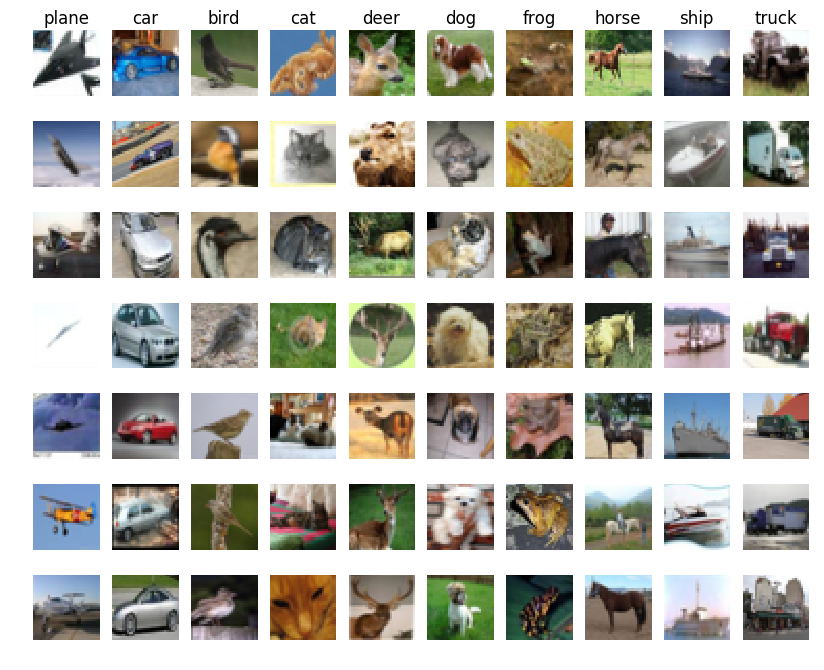
\includegraphics[scale=0.40]{methodology/figs/cifar10.png}}
    \caption{Classes in CIFAR-10}
    \label{fig:cifar10}
\end{figure}

\subsection{ImageNet ILSVRC 2012 Challenge}
ImageNet is an image dataset organized according to the WordNet hierarchy. Each 
meaningful concept in WordNet, possibly described by multiple words or word 
phrases, is called a "synonym set" or "synset". There are more than 100,000 
synsets in WordNet, majority of them are nouns (80,000+). ImageNet aims to 
provide on average 1000 images to illustrate each synset. Images of each concept 
are quality-controlled and human-annotated. In its completion, ImageNet will 
offer tens of millions of cleanly sorted images for most of the concepts in 
the WordNet hierarchy.

The ImageNet Large Scale Visual Recognition Challenge or ILSVRC for short is an 
annual competition helped between 2010 and 2017 in which challenge tasks use 
subsets of the ImageNet dataset.  The goal of the challenge was to both promote 
the development of better computer vision techniques and to benchmark the state 
of the art.
The annual challenge focuses on multiple tasks for image classification that 
includes both assigning a class label to an image based on the main object in 
the photograph and object detection that involves localizing objects within 
the photograph.

We use the dataset released from the 2012 challenge.  The validation and test 
data for this competition consists of 150,000 photographs, collected from flickr 
and other search engines, hand labeled with the presence or absence of 1000 
object categories. The 1000 object categories contain both internal nodes and 
leaf nodes of ImageNet, but do not overlap with each other. A random subset of 
50,000 of the images with labels is released as validation data. The remaining 
images are used for evaluation and are released without labels at test time.  
The training data, the subset of ImageNet containing the 1000 categories and 1.2 
million images. 
